%%%%%%%%%%%%%%%%%%%%%%%%%%%%%%%%%%%%%%%%%%%%%%%%%%%%%%%%%%%%%%%%%%%%%
%
%  This is a sample LaTeX input file for your contribution to 
%  the M&C2019 topical meeting.
%
%  Please use it as a template for your full paper 
%    Accompanying/related file(s) include: 
%       1. Document class/format file: mandc.cls
%       2. Sample Postscript Figure:   figure.pdf
%       3. A PDF file showing the desired appearance: mandc2019_template.pdf
%       4. cites.sty and citesort.sty that might be needed by some users 
%    Direct questions about these files to: palmert@engr.orst.edu
%											mark.dehart@inl.gov
%
%    Notes: 
%      (1) You can use the "dvips" utility to convert .dvi 
%          files to PostScript.  Then, use either Acrobat 
%          Distiller or "ps2pdf" to convert to PDF format. 
%      (2) Different versions of LaTeX have been observed to 
%          shift the page down, causing improper margins.
%          If this occurs, adjust the "topmargin" value in the
%          physor2018.cls file to achieve the proper margins. 
%
%%%%%%%%%%%%%%%%%%%%%%%%%%%%%%%%%%%%%%%%%%%%%%%%%%%%%%%%%%%%%%%%%%%%%


%%%%%%%%%%%%%%%%%%%%%%%%%%%%%%%%%%%%%%%%%%%%%%%%%%%%%%%%%%%%%%%%%%%%%
\documentclass[letterpaper]{mandc2019}
%
%  various packages that you may wish to activate for usage 
\usepackage{tabls}
\usepackage{graphicx}
\usepackage{cites}
\usepackage{epsf}
\usepackage{appendix}
\usepackage{ragged2e}
\usepackage[top=1in, bottom=1.in, left=1.in, right=1.in]{geometry}
\usepackage{enumitem}
\setlist[itemize]{leftmargin=*}
\usepackage{caption}
\captionsetup{width=1.0\textwidth,font={bf,normalsize},skip=0.3cm,within=none,justification=centering}
%\usepackage{float}
%Better boldface math font.
\usepackage{bm}
%Algorithm
\usepackage{algorithm}
\usepackage{algorithmic}
\usepackage{siunitx}
\usepackage[table]{xcolor}
\usepackage{placeins}



\newcommand{\tcr}[1]{\textcolor{red}{#1}}
\newcommand{\vr}{\vec{r}}
\newcommand{\vo}{\vec{\Omega}}

%\usepackage[justification=centering]{caption}

%
% Define title...
%
\title{APPROACHES TO LOAD BALANCING \\
MASSIVELY PARALLEL TRANSPORT SWEEPS\\
ON UNSTRUCTURED GRIDS}
%
% ...and authors
%
\author{%
  % FIRST AUTHORS 
  %
  \textbf{Tarek Habib Ghaddar$^1$, Jean C. Ragusa$^1$, Jan Vermaak$^1$, Marvin L. Adams$^1$} \\
$^1$Dept. of Nuclear Engineering, Texas  A\&M University \\
  College Station, TX, 77843-3133 \\ 
     \\
  \url{tghaddar@tamu.edu}, \url{jean.ragusa@tamu.edu}, \url{janv@tamu.edu}, \url{mladams@tamu.edu}
}
%
% Insert authors' names and short version of title in lines below
%
\newcommand{\authorHead}      % Author's names here use et al. if more than 3
           {First author}  
\newcommand{\shortTitle}      % Short title here (Shorten to fit all into a single line)
           {Paper Title }  
%%%%%%%%%%%%%%%%%%%%%%%%%%%%%%%%%%%%%%%%%%%%%%%%%%%%%%%%%%%%%%%%%%%%%
%
%   BEGIN DOCUMENT
%
%%%%%%%%%%%%%%%%%%%%%%%%%%%%%%%%%%%%%%%%%%%%%%%%%%%%%%%%%%%%%%%%%%%%%
\begin{document}
\maketitle
\justify 

\begin{abstract}
  Use 8.5$\times$11 paper size, with 1'' margins on all sides.  A required 200-250 
  word abstract starts on this line.  Leave two blank lines before ``ABSTRACT''
  and one after.  Use 11 point Times New Roman here and single 
  spacing. The abstract is a very brief summary highlighting main 
  accomplishments, what is new, and how it relates to the state-of-the-art.
\end{abstract}
\keywords{transport sweep, massively parallel, load balancing}

\section{INTRODUCTION} 
The steady-state neutron transport equation describes the behavior of neutrons in a medium and is given by Eq. (\ref{continuous transport}):
\begin{multline}
\vo \cdot \vec \nabla \psi(\vr,E,\vo) + \Sigma_t(\vr,E) \psi(\vr,E,\vo)  = \\ 
\int_{0}^{\infty}dE' \int_{4\pi}d\Omega' \Sigma_s(\vr,E'\to E, \Omega'\to\Omega)\psi(\vr,E',\vo')  + S_{ext}(\vr,E,\vo) ,
\label{continuous transport}
\end{multline}
where $\vec{\Omega}\cdot \vec\nabla\psi$ is the leakage term and $\Sigma_t\psi$ is the total collision term (absorption, outscatter, and within group scattering). These represent the loss terms of the neutron transport equation. The right hand side of Eq.~\eqref{continuous transport} represents the gain terms, where $S_{ext}$ is the external source of neutrons and $\int_{0}^{\infty}dE'\int_{4\pi}d\Omega'\Sigma_s(E'\to E, \Omega'\to\Omega)\psi(\vr,E',\vo')$ is the inscatter term, which represents all neutrons scattering from energy $E'$ and direction $\vo'$ into $dE$ about energy $E$ and $d\Omega$ about direction $\vo$. 

Eq. (\ref{angle}) is obtained by assuming isotropic scattering, discretizing in energy, and discretizing in angle using the discrete ordinates method\cite{discrete ordinates}:
\begin{equation}
\vo_m \cdot \vec \nabla \psi_{g,m}(\vr) +\Sigma_{t,g}(\vr) \psi_{g,m}(\vr)  = \frac{1}{4\pi}\sum_{g^{\prime}}\Sigma_{s,g^{\prime}\to g}(\vr)\phi_{g^{\prime}}(\vr) + S_{ext,g,m}(\vr).
\label{angle}
\end{equation}
This allows us to solve a sequence of transport equations for one group and direction at a time. The discrete form of the transport equation is solved via source iteration, described in Eq. (\ref{source iteration}):
\begin{equation}
\vo_m \cdot \vec\nabla \psi_m^{(l+1)}(\vr) + \Sigma_t \psi_m^{(l+1)}(\vr) = q_m^{(l)}(\vr),
\label{source iteration}
\end{equation}
where the gain terms terms have been combined into one general source term, $q_m$. The angular flux of iteration $(l+1)$ is calculated using the $(l^{th})$ value of the scalar flux. 

After the angular and energy dependence have been accounted for, Eq. (\ref{source iteration}) must be discretized in space as well. This is done by meshing the domain and utilizing one of three popular discretization techniques: finite difference\cite{fd}, finite volume\cite{fd}, or discontinuous finite element\cite{Reed}, allowing one cell at a time to be solved. The solution across a cell interface is connected based on an upwind approach, where face outflow radiation becomes face inflow radiation for the downwind cells. 

PDT, Texas A\&M's massively parallel deterministic transport code, employs the transport sweep with the process described above, using a finite element mesh and solving the discrete ordinates form of the transport equation using a discontinuous finite element approach and source iteration\cite{mpadams15, mpadams13}. Initially, PDT only swept on structured, logically Cartesian meshes. As the need to solve problems with more complex geometries arose, PDT added a support for arbitrary polyhedral unstructured meshes. However, this introduced imbalanced partitions, causing longer and unmanageable runtimes.

To combat imbalanced partitions, two load balancing algorithms were implemented, referred to in this paper as the original load balancing algorithm and the load balancing by dimension algorithm.

\section{LOAD BALANCING UNSTRUCTURED MESHES IN PDT} 
\label{sec:first}

Before detailing the two load balancing algorithms PDT employs, a quick review of partitioning unstructured meshes in PDT is necessary:
%\vspace{-2.5cm}
\begin{itemize}\itemsep 1pt \parskip 0pt \parsep 0pt
\item ``Cut lines" in 2D (cut planes for 3D) are used to slice through the mesh in the $x$, $y$, and $z$ dimensions.
\item The cut planes form brick partitions, called subsets, that have unstructured meshes inside of them. 
\item The subsets are distributed amongst the processor domain.
\end{itemize}
%\vspace{-2cm}
Figure \ref{partitioning_example} shows an example of an unstructured mesh partitioned into four subsets in PDT. 

\begin{figure}[!htb]
\centering
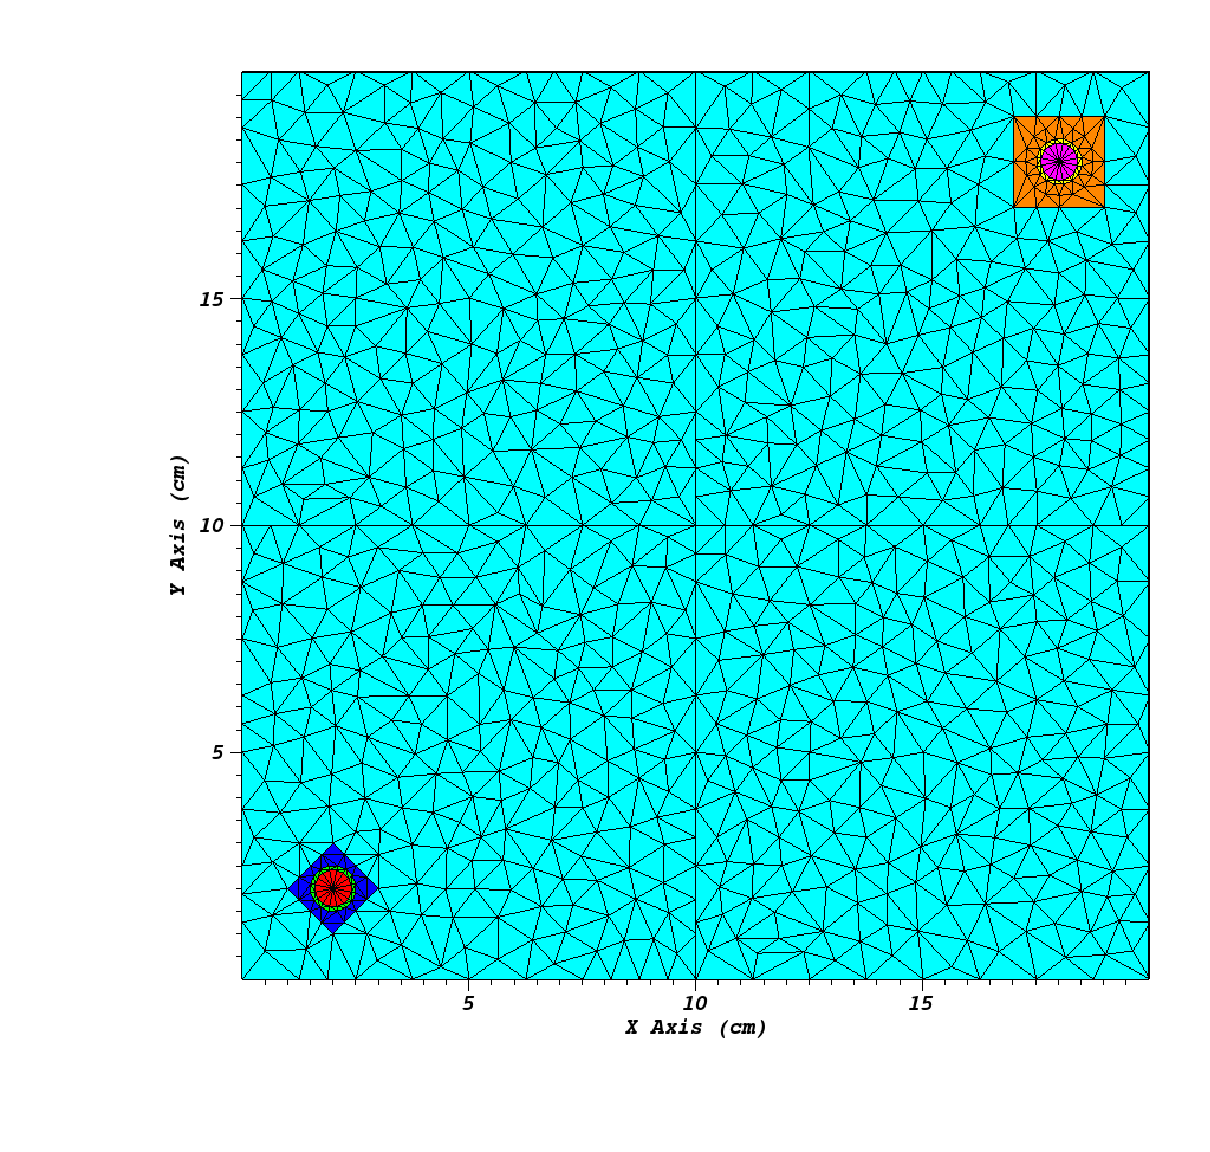
\includegraphics[scale=0.9,trim={0.95in 0.64in 0.35in 0.44in},clip]{Figures/partitioning_example.pdf}
\caption{An unstructured mesh partitioned into four subsets with cut lines at $\bm{x,y = 10}$ cm.}
\label{partitioning_example}
\end{figure}
Both approaches to load balancing move these cut lines in order to redistribute cells more evenly throughout subsets. We define a metric describing how imbalanced our problem is:
\begin{equation}
f =\frac{\underset{ijk}{\text{max}}(N_{ijk})}{\frac{N_{tot}}{I\cdot J\cdot K}},
\label{metric_def}
\end{equation}
where $f$ is the load balance metric, $N_{ijk}$ is the number of cells in subset $(i,j,k)$, $N_{tot}$ is the global number of cells in the problem, and $I$, $J$, and $K$ are the total number of subsets in the $x$, $y$, and $z$ direction, respectively. The metric is a measure of the maximum number of cells per subset divided by the average number of cells per subset. For a perfectly balanced problem, $f = 1$.

Dimensional sub-metrics are defined to assist with the movement of the partitions:
\begin{equation}
f_{D} = \underset{d}{\text{max}}[\sum_{d2,d3} N_{ijk}]/\frac{N_{tot}}{D}.
\label{f_d}
\end{equation}
$f_{D}$ is calculated by taking the maximum number of cells per row, column, or plane and dividing it by the average number of cells per the corresponding dimension. If this number is greater than predefined tolerances, the cut lines in the respective dimension are redistributed. 

Figure \ref{redistribute} illustrates an example of redistributing the cut lines in $x$ to balance the cells per column.
\begin{figure}[!htb]
\centering
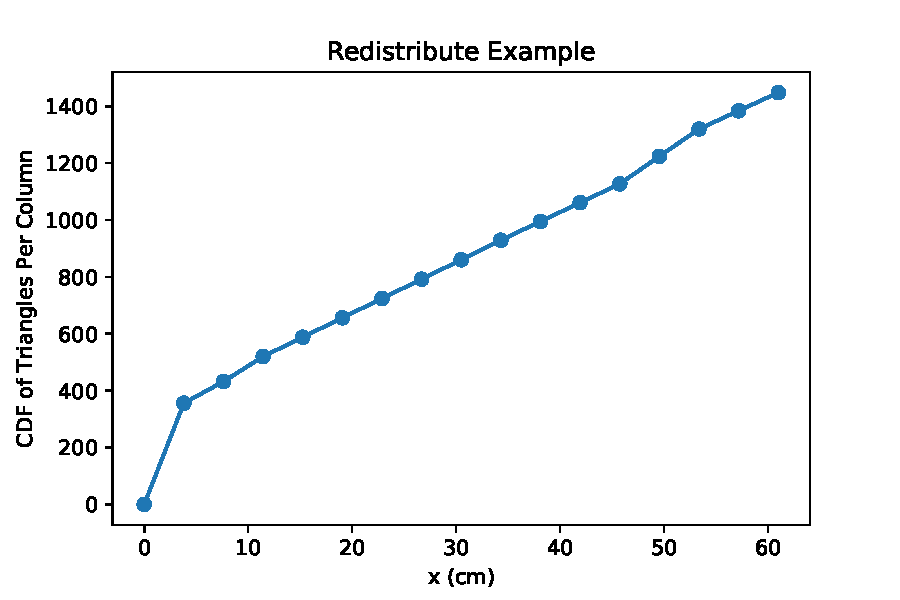
\includegraphics[scale=0.5]{Figures/redistribute_before.pdf}
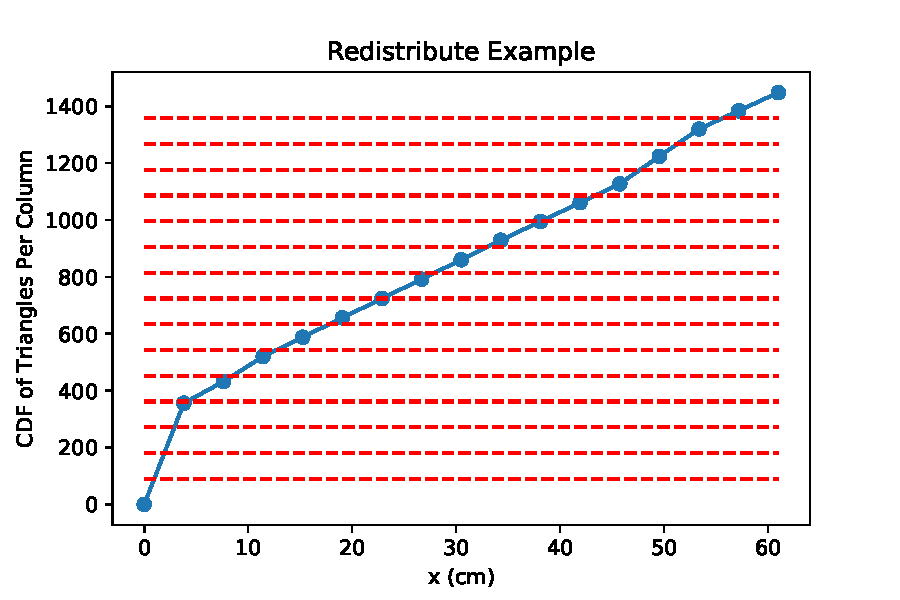
\includegraphics[scale=0.5]{Figures/redistribute_after.pdf}
\caption{The use of the CDF of triangles per column to redistribute the cut lines in X.}
\label{redistribute}
\end{figure}
The image on the left side of Fig. \ref{redistribute} shows the CDF of the triangles per column. The red lines on the right side of Fig. \ref{redistribute} show the ideal equal number of cells per column. The x-value of the intersection of these red lines and the CDF are where the cut lines are redistributed to. 

\subsection{Original Load Balancing Algorithm}
\label{og_lb}

The initial approach to load balancing was implemented on 2D extruded meshes, meaning the mesh is balanced in the 2D plane and then extruded, yielding a balanced 3D mesh. Algorithm \ref{initial_algorithm} summarizes the initial approach to load balancing meshes in PDT.

\begin{algorithm}[!htb]
\caption{The original load balancing algorithm.}
\label{initial_algorithm}
\begin{algorithmic}

\WHILE{$f > \text{tol}_{\text{subset}}$}
  \IF {$f_I > \text{tol}_{\text{col}}$}
    \STATE Redistribute the X cut lines.
  \ENDIF
  \IF {$f_J > \text{tol}_{\text{row}}$}
  	\STATE Redistribute the Y cut lines.
  \ENDIF
\ENDWHILE
\end{algorithmic}
\end{algorithm}
While the problem is not balanced, we check if the cells per column and cells per row, represented by $f_I$ and $f_J$ (defined by Eq. (\ref{f_d})), are balanced. If they are not, we redistribute the cut lines. 
%\vspace{-3.5cm}

This initial approach involved placing cut lines in all dimensions all the way through the mesh. This created an orthogonal partitioning where each subset had an equivalent number of neighbors, which was done to preserve the optimal sweep partitioning described by Adams et. al \cite{mpadams2015}. However, there are theoretical limits to load balancing in this fashion. Figure \ref{2dgeneral} shows a simple 2D subset layout with $M$ unaligned patches of high mesh density.

\begin{figure}[H]
\centering
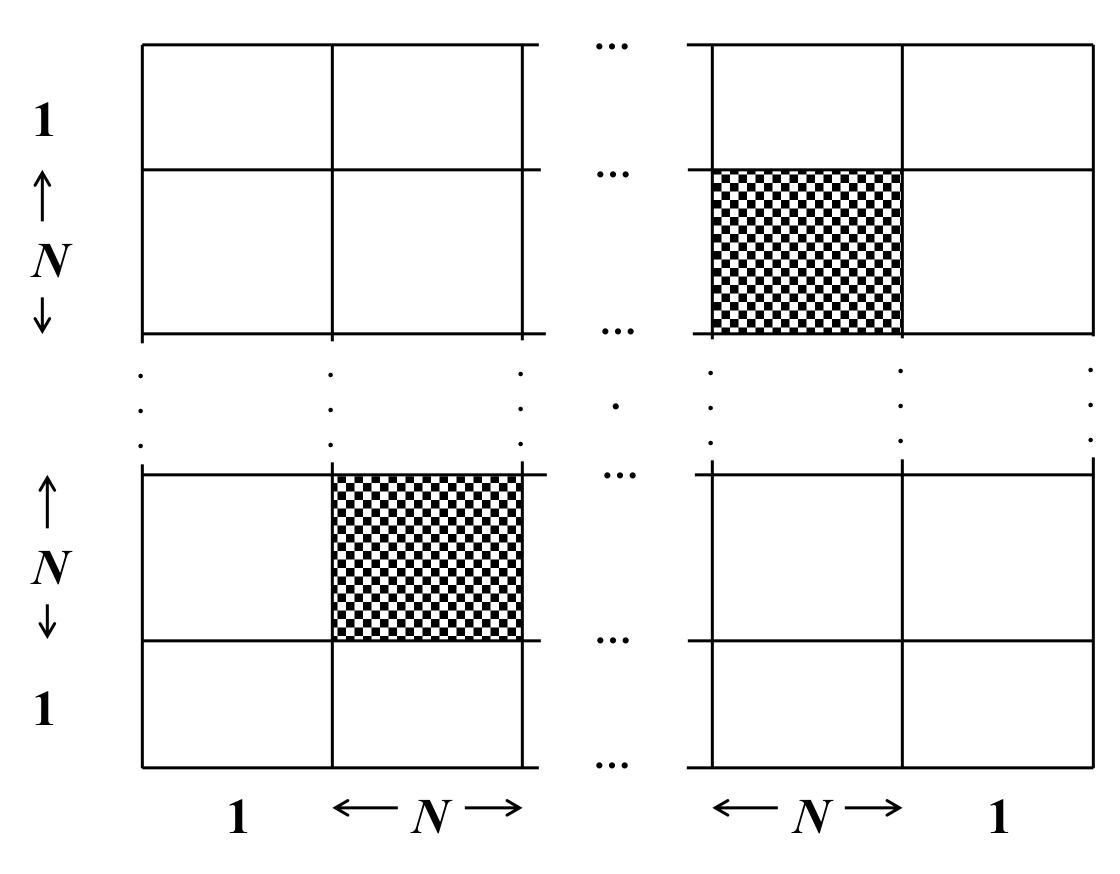
\includegraphics[scale=0.6]{figures/2dgeneral.png}
\caption{A 2D subset layout with $M$ unaligned patches of high mesh density.}
\label{2dgeneral}
\end{figure}

The subset layout is $[M(N+1)+1] \times [M(N+1)+1]$, but only $MN^2$ subset have significant work, leading to a theoretical limit for the load imbalance factor:
\begin{equation}
f= \frac{\left( M(N+1)+1 \right)^2}{MN^2} \xrightarrow{N\to \infty} \frac{M^2N^2}{MN^2} = M.
\end{equation}

Due to this theoretical limit, the load balancing by dimension algorithm was developed.

\subsection{Load Balancing by Dimension Algorithm}

The load balancing by dimension algorithm, like the original load balancing algorithm, relies on the movement of cut planes to redistribute mesh cells in a more balanced manner. However rather than moving all cut planes in all dimensions in one iteration, one dimension is balanced first for all iterations, and then the cut planes that yield the best metric for that dimension are chosen. Then the next dimensions is balanced within the first dimension. For example, if the $x$ cut planes are balanced first, the $y$ cut planes are balanced \textit{within} each column.
We slightly alter the definition for our dimensional sub-metrics (Eq. (\ref{f_d})) accordingly:
\begin{align}
f_{D1} &= \underset{d1}{\text{max}}[\sum_{d2,d3} N_{ijk}]/\frac{N_{tot}}{D1}, \label{f_d1} \\
f_{D2,d1} &= \Big(\underset{d2}{\text{max}}[\sum_{d3} N_{ijk,d1}]/\frac{N_{d1}}{D2}\Big), \label{f_d2}\\
f_{D3,d2,d1} &= \Big( \underset{d3}{\text{max}}[ N_{ijk,d1,d2}]/\frac{N_{d1,d2}}{D3} \Big) . \label{f_d3}
\end{align}
Equation (\ref{f_d1}) represents the sub-metric for the first dimension we load balance. In order to assist in the explanation of $f_{D2,d1}$ and $f_{D3,d2,d1}$, we'll take $D1$ to be the $z$ dimension. In Eq. ({\ref{f_d1}), $D1$ represents the number of $z$ planes, $N_{tot}$ represents the number of cells in the mesh, and $N_{ijk}$ is the number of cells in subset $(i,j,k)$. $f_{D1}$ is the maximum number of cells per plane by the average number of cells per plane. 

Once the z planes are balanced according to $f_{D1}$, we balance the second dimension (in this example, the columns, or $x$ cut planes) \textit{within} each $z$ plane. $f_{D2,d1}$ represents the column-wise sub-metrics for each $z$ plane. In other words, there are $D1$ column-wise sub-metrics, one for each plane. These column-wise sub-metrics are calculated by dividing the maximum number of cells per column divided by the average number cells per column \textit{in each plane}. 

Once the columns within each z-plane are balanced, we balance the rows $within$ the columns $within$ each plane. The row-wise sub-metrics for each plane for each column, $f_{D3,d2,d1}$, are calculated by dividing the maximum number of cells per row per column by the average number of cells per row per column in each plane. Algorithm \ref{lbd} summarizes the load balancing by dimension process described.

\begin{algorithm}[!htb]
\caption{The load balancing by dimension algorithm.}
\label{lbd}
\begin{algorithmic}

  \WHILE {$f_{D1} > \text{tol}_{\text{D1}}$}
    \STATE Redistribute the D1 cut planes.
  \ENDWHILE  
  
  \FOR {$d1$ in $D1$}
    \WHILE {$f_{D2,d1} > \text{tol}_{\text{D2}}$}
      \STATE Redistribute the D2 cut planes within d1. 
    \ENDWHILE
  \ENDFOR
  
  \FOR{$d1$ in $D1$}
    \FOR{$d2$ in $D2$}
      \WHILE {$f_{D3,d2,d1} > \text{tol}_{\text{D3}}$ }
        \STATE Redistribute the D3 cut planes within d2 within d1. 
      \ENDWHILE
    \ENDFOR
  \ENDFOR
  
  \STATE Calculate $f$.
\end{algorithmic}
\end{algorithm}

\section{RESULTS}

To study the behavior of the original load balancing algorithm and the load balancing by dimension algorithm, the problem shown in Fig. \ref{partitioning_example} was run with a varying number of subsets and with a varying maximum triangle area, with the minimum allowable angle per triangle was kept constant at \ang{20}. We varied the number of subsets in $x$ and $y$ from 2 to 10 (with the total number of subsets varying from 4 to 100). The problem illustrated by Fig. \ref{partitioning_example} was chosen because it has two dense features in opposing corners with no features in between, lending itself to being an imbalanced mesh. Table \ref{og_table} shows the results of this parametric study using the original load balancing algorithm vs. using the load balancing by dimension algorithm. Table \ref{all_improvements} shows the percent improvements for both algorithms from no load balancing to running both load balancing algorithm, while Table \ref{method_improvement} shows the improvement of the load balancing by dimension algorithm relative to the original load balancing algorithm.
%\vspace{-1cm}
\begin{table}[!htb]
\centering
  \caption{\bf The results of the parametric study using the original load balancing algorithm (left) and the load balancing by dimension algorithm (right).}
  \scalebox{0.5}{
  \begin{tabular}{c|c|c|c|c|c|c|c|c|c} 
  \bf Area, $N^{1/2}$ & \bf  2 &  \bf 3    &  \bf  4   &  \bf  5   &  \bf  6   &  \bf  7   & \bf   8   &  \bf 9    &  \bf 10   \\ \hline \hline
\bf Coarse&1.993 & 2.735 & 4.360 & 4.812 & 5.545 & 6.321 & 3.114 & 2.697 & 1.893 \\ \hline 
\bf 1.8& 1.408 & 2.277 & 2.886 & 3.269 & 4.716 & 4.721 & 5.890 & 4.618 & 1.863 \\ \hline
\bf 1.6& 1.375 & 2.206 & 2.649 & 3.247 & 4.356 & 4.876 & 4.678 & 5.062 & 1.329 \\ \hline
\bf 1.4& 1.337 & 2.110 & 2.982 & 3.031 & 4.615 & 4.310 & 8.911 & 4.652 & 2.675 \\ \hline
\bf 1.2& 1.344 & 2.008 & 2.017 & 3.392 & 3.916 & 4.969 & \cellcolor{blue!25}9.576 & 4.543 & 4.728 \\ \hline
\bf 1.0& 1.264 & 1.806 & 2.405 & 2.976 & 3.657 & 4.317 & 6.242 & 4.831 & 4.941 \\ \hline
\bf 0.8& 1.212 & 1.640 & 2.300 & 2.436 & 2.941 & 4.395 & 7.420 & 4.466 & 3.947 \\ \hline
\bf 0.6& 1.153 & 1.567 & 2.045 & 2.368 & 3.199 & 2.999 & 7.206 & 4.101 & 3.592 \\ \hline
\bf 0.4& 1.108 & 1.411 & 1.633 & 2.117 & 2.383 & 2.646 & 6.970 & 3.086 & 2.511 \\ \hline
\bf 0.2& 1.052 & 1.197 & 1.258 & 1.523 & 1.789 & 1.857 & 3.380 & 2.193 & 1.883 \\ \hline
\bf 0.1& 1.029 & 1.092 & 1.149 & 1.207 & 1.276 & 1.420 & 2.015 & 1.565 & 1.247 \\ \hline
\bf 0.08& 1.009 & 1.043 & 1.086 & 1.101 & 1.179 & 1.267 & 2.118 & 1.551 & 1.271 \\ \hline
\bf 0.06& 1.009 & 1.024 & 1.059 & 1.094 & 1.138 & 1.154 & 1.825 & 1.432 & 1.138 \\ \hline
\bf 0.05& 1.008 & 1.023 & 1.025 & 1.028 & 1.073 & 1.149 & 1.666 & 1.380 & 1.110 \\ \hline
\bf 0.04& 1.005 & 1.016 & 1.017 & 1.021 & 1.038 & 1.051 & 1.520 & 1.311 & 1.080 \\ \hline
\bf 0.03& 1.005 & 1.008 & 1.018 & 1.039 & 1.059 & 1.073 & 1.450 & 1.179 & \cellcolor{red!25}1.001 \\ \hline
\bf 0.02& 1.005 & 1.008 & 1.010 & 1.013 & 1.021 & 1.035 & 1.623 & 1.137 & 1.016 \\ \hline
\bf 0.01& 1.003 & 1.009 & 1.009 & 1.011 & 1.016 & 1.013 & 1.281 & 1.058 & 1.015 \\ \hline
  \end{tabular}}
 \scalebox {0.5}{
   \begin{tabular}{c|c|c|c|c|c|c|c|c|c} 
\bf Area, $N^{1/2}$ & \bf  2 & \bf 3    &  \bf  4   &  \bf  5   &  \bf 6    &  \bf  7   &   \bf 8   &  \bf 9    &  \bf 10   \\ \hline \hline
\bf Coarse & 1.645 & 1.455 & 1.878 & 2.348 & 3.046 & 3.022 & 1.752 & 2.304 & 1.451 \\ \hline 
\bf 1.8& 1.034 & 1.460 & 2.127 & 1.744 & 2.098 & 2.588 & 2.623 & 2.776 & 2.872 \\ \hline
\bf 1.6& 1.015 & 1.396 & 1.899 & 1.877 & 2.090 & 2.857 & 2.608 & 3.582 & 2.604 \\ \hline
\bf 1.4& 1.011 & 1.418 & 1.631 & 1.964 & 1.820 & 2.968 & 2.055 & 2.201 & 1.523 \\ \hline
\bf 1.2& 1.019 & 1.344 & 1.483 & 1.983 & 2.122 & 3.023 & 2.356 & \cellcolor{blue!25}4.765 & 2.371 \\ \hline
\bf 1.0& 1.007 & 1.338 & 1.641 & 2.313 & 3.097 & 2.098 & 2.563 & 2.808 & 2.637 \\ \hline
\bf 0.8& 1.016 & 1.157 & 1.457 & 1.982 & 1.881 & 2.340 & 2.283 & 3.513 & 3.947 \\ \hline
\bf 0.6& 1.012 & 1.111 & 1.199 & 1.598 & 1.901 & 1.791 & 2.330 & 3.005 & 3.719 \\ \hline
\bf 0.4& 1.005 & 1.024 & 1.204 & 1.288 & 1.665 & 1.492 & 1.660 & 2.528 & 2.511 \\ \hline
\bf 0.2& 1.007 & 1.021 & 1.025 & 1.116 & 1.175 & 1.358 & 1.478 & 1.624 & 1.837 \\ \hline
\bf 0.1& 1.003 & 1.019 & 1.024 & 1.019 & 1.092 & 1.122 & 1.161 & 1.087 & 1.247 \\ \hline
\bf 0.08& 1.007 & 1.010 & 1.022 & 1.035 & 1.035 & 1.077 & 1.176 & 1.135 & 1.219 \\ \hline
\bf 0.06& 1.004 & 1.009 & 1.021 & 1.032 & 1.031 & 1.070 & 1.102 & 1.080 & 1.072 \\ \hline
\bf 0.05& 1.002 & 1.005 & 1.019 & 1.023 & 1.038 & 1.071 & 1.096 & 1.094 & 1.101 \\ \hline
\bf 0.04& 1.002 & 1.008 & 1.008 & 1.021 & 1.027 & 1.028 & 1.063 & 1.091 & 1.080 \\ \hline
\bf 0.03& 1.003 & 1.008 & 1.013 & 1.014 & 1.030 & 1.044 & 1.068 & 1.074 & \cellcolor{red!25}1.001 \\ \hline
\bf 0.02& 1.002 & 1.006 & 1.009 & 1.013 & 1.020 & 1.030 & 1.038 & 1.058 & 1.016 \\ \hline
\bf 0.01& \cellcolor{red!25}1.001 & 1.006 & 1.007 & 1.011 & 1.015 & 1.013 & 1.030 & 1.029 & 1.015 \\ \hline

  \end{tabular}} 
  \label{og_table}
\end{table}

\begin{table}[!htb]
\centering
\caption{\bf The percent improvement of the original load balancing algorithm (left) and the load balancing by dimension algorithm (right).}
\scalebox{0.5}{
\begin{tabular}{c|c|c|c|c|c|c|c|c|c} 

\bf Area, $N^{1/2}$ & \bf  2 & \bf 3    &  \bf  4   &  \bf  5   &  \bf 6    &  \bf  7   &   \bf 8   &  \bf 9    &  \bf 10   \\ \hline \hline
\bf Coarse& 0.000 & 0.367 & 0.403 & 0.552 & 0.628 & 0.491 & 0.890 & 0.720 & 0.765 \\ \hline 
 \bf 1.8& 0.000 & 0.091 & 0.337 & 0.364 & 0.473 & 0.390 & 0.767 & 0.413 & 0.683 \\ \hline 
 \bf 1.6& 0.000 & 0.093 & 0.398 & 0.368 & 0.499 & 0.370 & 0.815 & 0.353 & 0.774 \\ \hline 
 \bf 1.4& 0.000 & 0.061 & 0.080 & 0.410 & 0.415 & 0.412 & 0.570 & 0.413 & 0.545 \\ \hline 
 \bf 1.2& 0.000 & 0.007 & 0.391 & 0.340 & 0.378 & 0.315 & 0.536 & 0.245 & 0.196 \\ \hline 
 \bf 1.0& 0.000 & 0.038 & 0.206 & 0.420 & 0.341 & 0.186 & 0.696 & 0.201 & 0.160 \\ \hline 
 \bf 0.8& 0.000 & 0.049 & 0.109 & 0.336 & 0.434 & 0.139 & 0.637 & 0.228 & 0.000 \\ \hline 
 \bf 0.6& 0.000 & 0.000 & 0.057 & 0.199 & 0.163 & 0.346 & 0.517 & 0.000 & 0.090 \\ \hline 
 \bf 0.4& 0.000 & 0.000 & 0.065 & 0.013 & 0.267 & 0.147 & 0.528 & 0.179 & 0.000 \\ \hline 
 \bf 0.2& 0.000 & 0.000 & 0.000 & 0.000 & 0.001 & 0.041 & 0.566 & 0.121 & 0.000 \\ \hline 
 \bf 0.1& 0.000 & 0.000 & 0.000 & 0.000 & 0.000 & 0.000 & 0.540 & 0.089 & 0.000 \\ \hline 
 \bf 0.08&0.000 & 0.000 & 0.000 & 0.000 & 0.000 & 0.000 & 0.458 & 0.000 & 0.000 \\ \hline 
 \bf 0.06&0.000 & 0.000 & 0.000 & 0.000 & 0.000 & 0.000 & 0.409 & 0.000 & 0.000 \\ \hline 
 \bf 0.05&0.000 & 0.000 & 0.000 & 0.000 & 0.000 & 0.000 & 0.360 & 0.000 & 0.000 \\ \hline 
 \bf 0.04&0.000 & 0.000 & 0.000 & 0.000 & 0.000 & 0.000 & 0.348 & 0.000 & 0.000 \\ \hline 
 \bf 0.03&0.000 & 0.000 & 0.000 & 0.000 & 0.000 & 0.000 & 0.293 & 0.000 & 0.000 \\ \hline 
 \bf 0.02&0.000 & 0.000 & 0.000 & 0.000 & 0.000 & 0.000 & 0.000 & 0.000 & 0.000 \\ \hline 
 \bf 0.01&0.000 & 0.000 & 0.000 & 0.000 & 0.000 & 0.000 & 0.000 & 0.000 & 0.000 \\ \hline 
\end{tabular}}
\scalebox{0.5}{
\begin{tabular}{c|c|c|c|c|c|c|c|c|c} 
\bf Area, $N^{1/2}$ & \bf  2 & \bf 3    &  \bf  4   &  \bf  5   &  \bf 6    &  \bf  7   &   \bf 8   &  \bf 9    &  \bf 10   \\ \hline \hline
\bf Coarse& 0.175 & 0.663 & 0.743 & 0.781 & 0.796 & 0.757 & 0.938 & 0.760 & 0.820 \\ \hline 
  \bf 1.8& 0.266 & 0.417 & 0.511 & 0.661 & 0.766 & 0.665 & 0.896 & 0.647 & 0.512 \\ \hline 
  \bf 1.6& 0.262 & 0.426 & 0.568 & 0.635 & 0.760 & 0.631 & 0.897 & 0.542 & 0.557 \\ \hline 
  \bf 1.4& 0.244 & 0.369 & 0.497 & 0.618 & 0.769 & 0.595 & 0.901 & 0.722 & 0.741 \\ \hline 
  \bf 1.2& 0.242 & 0.336 & 0.552 & 0.614 & 0.663 & 0.583 & 0.886 & 0.208 & 0.597 \\ \hline 
  \bf 1.0& 0.203 & 0.287 & 0.458 & 0.549 & 0.442 & 0.605 & 0.875 & 0.536 & 0.552 \\ \hline 
  \bf 0.8& 0.162 & 0.330 & 0.435 & 0.460 & 0.638 & 0.542 & 0.888 & 0.393 & 0.000 \\ \hline 
  \bf 0.6& 0.122 & 0.291 & 0.447 & 0.460 & 0.503 & 0.610 & 0.844 & 0.267 & 0.058 \\ \hline 
  \bf 0.4& 0.093 & 0.274 & 0.310 & 0.400 & 0.488 & 0.519 & 0.888 & 0.328 & 0.000 \\ \hline 
  \bf 0.2& 0.042 & 0.147 & 0.185 & 0.267 & 0.344 & 0.299 & 0.810 & 0.349 & 0.025 \\ \hline 
  \bf 0.1& 0.026 & 0.067 & 0.109 & 0.156 & 0.144 & 0.210 & 0.735 & 0.367 & 0.000 \\ \hline 
  \bf 0.08&0.002 & 0.032 & 0.059 & 0.060 & 0.122 & 0.150 & 0.699 & 0.268 & 0.041 \\ \hline 
  \bf 0.06&0.005 & 0.014 & 0.036 & 0.057 & 0.094 & 0.073 & 0.643 & 0.246 & 0.058 \\ \hline 
  \bf 0.05&0.006 & 0.017 & 0.006 & 0.005 & 0.033 & 0.068 & 0.579 & 0.208 & 0.008 \\ \hline 
  \bf 0.04&0.002 & 0.008 & 0.009 & 0.000 & 0.011 & 0.022 & 0.544 & 0.168 & 0.000 \\ \hline 
  \bf 0.03&0.002 & 0.000 & 0.005 & 0.024 & 0.028 & 0.027 & 0.479 & 0.089 & 0.000 \\ \hline 
  \bf 0.02&0.003 & 0.002 & 0.001 & 0.000 & 0.001 & 0.004 & 0.361 & 0.070 & 0.000 \\ \hline 
  \bf 0.01&0.002 & 0.003 & 0.002 & 0.000 & 0.001 & 0.000 & 0.196 & 0.027 & 0.000 \\ \hline 

\end{tabular}}
\label{all_improvements}
\end{table}

%method improvement table
\begin{table}[!htb]
\centering
\caption{\bf The percent improvement of the load balancing by dimension algorithm over the original load balancing algorithm.}
\scalebox{0.75}{
\begin{tabular}{c|c|c|c|c|c|c|c|c|c} 
\bf Area, $N^{1/2}$ & \bf  2 & \bf 3    &  \bf  4   &  \bf  5   &  \bf 6    &  \bf  7   &   \bf 8   &  \bf 9    &  \bf 10   \\ \hline \hline
\bf Coarse&  0.175 & 0.663 & 0.743 & 0.781 & 0.796 & 0.757 & 0.938 & 0.760 & 0.820 \\ \hline 
\bf 1.8&  0.266 & 0.417 & 0.511 & 0.661 & 0.766 & 0.665 & 0.896 & 0.647 & 0.512 \\ \hline 
\bf 1.6&  0.262 & 0.426 & 0.568 & 0.635 & 0.760 & 0.631 & 0.897 & 0.542 & 0.557 \\ \hline 
\bf 1.4&  0.244 & 0.369 & 0.497 & 0.618 & 0.769 & 0.595 & 0.901 & 0.722 & 0.741 \\ \hline 
\bf 1.2&  0.242 & 0.336 & 0.552 & 0.614 & 0.663 & 0.583 & 0.886 & 0.208 & 0.597 \\ \hline 
\bf 1.0&  0.203 & 0.287 & 0.458 & 0.549 & 0.442 & 0.605 & 0.875 & 0.536 & 0.552 \\ \hline 
\bf 0.8&  0.162 & 0.330 & 0.435 & 0.460 & 0.638 & 0.542 & 0.888 & 0.393 & 0.000 \\ \hline 
\bf 0.6&  0.122 & 0.291 & 0.447 & 0.460 & 0.503 & 0.610 & 0.844 & 0.267 & 0.058 \\ \hline 
\bf 0.4&  0.093 & 0.274 & 0.310 & 0.400 & 0.488 & 0.519 & 0.888 & 0.328 & 0.000 \\ \hline 
\bf 0.2&  0.042 & 0.147 & 0.185 & 0.267 & 0.344 & 0.299 & 0.810 & 0.349 & 0.025 \\ \hline 
\bf 0.1&  0.026 & 0.067 & 0.109 & 0.156 & 0.144 & 0.210 & 0.735 & 0.367 & 0.000 \\ \hline 
\bf 0.08& 0.002 & 0.032 & 0.059 & 0.060 & 0.122 & 0.150 & 0.699 & 0.268 & 0.041 \\ \hline 
\bf 0.06& 0.005 & 0.014 & 0.036 & 0.057 & 0.094 & 0.073 & 0.643 & 0.246 & 0.058 \\ \hline 
\bf 0.05& 0.006 & 0.017 & 0.006 & 0.005 & 0.033 & 0.068 & 0.579 & 0.208 & 0.008 \\ \hline 
\bf 0.04& 0.002 & 0.008 & 0.009 & 0.000 & 0.011 & 0.022 & 0.544 & 0.168 & 0.000 \\ \hline 
\bf 0.03& 0.002 & 0.000 & 0.005 & 0.024 & 0.028 & 0.027 & 0.479 & 0.089 & 0.000 \\ \hline 
\bf 0.02& 0.003 & 0.002 & 0.001 & 0.000 & 0.001 & 0.004 & 0.361 & 0.070 & 0.000 \\ \hline 
\bf 0.01& 0.002 & 0.003 & 0.002 & 0.000 & 0.001 & 0.000 & 0.196 & 0.027 & 0.000 \\ \hline 
\end{tabular}}
\label{method_improvement}
\end{table}

\FloatBarrier
\section{CONCLUSIONS AND FUTURE WORK}

Present your summary and conclusions here.

\section*{ACKNOWLEDGEMENTS}

Acknowledge the help of colleagues and sources of funding, as appropriate.

\textbf{As an example:} The format for this template was adapted from the \LaTeX template for the PHYSOR-2018 conference posted and available on the Internet and 
most of the \LaTeX\ format definitions contained in this were already defined. The 
M\&C 2019 organizing committee deeply thank the PHYSOR-2018 technical committee 
for this great support.

% You can enter a bibliography into the document using the following format, or use the 
% bibliography style file "mandc.bst" found in the template directory.  You can use the bibliography style file
% by replacing the current bibliography block with:
% \setlength{\baselineskip}{12pt}
% \bibliographystyle{mandc}
% \bibliography{mandc}

\setlength{\baselineskip}{12pt}
\begin{thebibliography}{300}
\bibitem{journal} B. Author(s), ``Title,'' \emph{Journal Name in Italic}, 
  \textbf{Volume in Bold}, pp. 34-89 (19xx).
\bibitem{proc_paper} C. D. Author(s), ``Article Title,'' \emph{Proceedings of
  Meeting in Italic}, Location, Dates of Meeting, Vol. n, pp. 134-156 
  (19xx).
\bibitem{book} E. F. Author, \emph{Book Title in Italic}, Publisher, City \&
  Country (19xx). 
\bibitem{website} ``Spallation Neutron Source: The next-generation 
  neutron-scattering facility in the United States,'' 
  \url{http://www.sns.gov/documentation/sns\_brochure.pdf} (2002).
\end{thebibliography}

\appendix
\gdef\thesection{APPENDIX \Alph{section}}
\section{Sample Appendix 1}
\label{app:a}
If necessary, include Appendices numbered in upper case alphabetical order. This is \ref{app:a}. 



\end{document}
